%%%%%%%%%%%%%%%%%%%%%%%%%%%%%%%%%%%%%%%%%%%%%%%%%%%%%%%%%%%%%%%%%%%%
%% I, the copyright holder of this work, release this work into the
%% public domain. This applies worldwide. In some countries this may
%% not be legally possible; if so: I grant anyone the right to use
%% this work for any purpose, without any conditions, unless such
%% conditions are required by law.
%%%%%%%%%%%%%%%%%%%%%%%%%%%%%%%%%%%%%%%%%%%%%%%%%%%%%%%%%%%%%%%%%%%%

\documentclass{beamer}
%%%%%%%%%%%%%%%%%%%%%%%%%%%%%%%%%%%%%%%%%%%%%%%%%%%%%%%%%%%%%%%%%%%%%%%%%%%%%%%%%%%%%%%
% Packages Definition
%%%%%%%%%%%%%%%%%%%%%%%%%%%%%%%%%%%%%%%%%%%%%%%%%%%%%%%%%%%%%%%%%%%%%%%%%%%%%%%%%%%%%%%
\usepackage[toc,page]{appendix}
\usetheme[faculty=science, university=uu, logo=uu-logo]{fibeamer}
\usepackage[main=english]{babel}
\usepackage{hyperref}
\usepackage{pgf,pgfpages}
\usepackage{graphicx}
\usepackage{units}
\usepackage[utf8]{inputenc}
\usepackage{multicol}
\usepackage{xspace}
\usepackage{textcomp}% for '\textdegree' macro
\usepackage{utopia} %font utopia imported
\usepackage{fontawesome}
\usepackage[center]{caption}
\usepackage{subcaption}
\usepackage{gensymb}
\usepackage{adjustbox}
\usepackage{marginnote}
\usepackage{textpos}
\usepackage[default]{lato}
\overfullrule=2cm

%%%%%%%%%%%%%%%%%%%%%%%%%%%%%%%%%%%%%%%%%%%%%%%%%%%%%%%%%%%%%%%%%%%%%%%%%%%%%%%%%%%%%%%
\beamertemplatenavigationsymbolsempty
%%%%%%%%%%%%%%%%%%%%%%%%%%%%%%%%%%%%%%%%%%%%%%%%%%%%%%%%%%%%%%%%%%%%%%%%%%%%%%%%%%%%%%%
\AtBeginSection[]{
	\begin{frame}[c]
	\vfill
	\centering
	\begin{beamercolorbox}[sep=8pt,center,shadow=false,rounded=true]{title}
		\usebeamerfont{title} \secname\par%
	\end{beamercolorbox}
	\vfill
\end{frame}
}

%%%%%%%%%%%%%%%%%%%%%%%%%%%%%%%%%%%%%%%%%%%%%%%%%%%%%%%%%%%%%%%%%%%%%%%%%%%
\newcommand\Wider[2][3em]{%
	\makebox[\linewidth][c]{%
		\begin{minipage}{\dimexpr\textwidth+#1\relax}
			\raggedright#2
		\end{minipage}%
	}%
}

%%%%%%%%%%%%%%%%%%%%%%%%%%%%%%%%%%%%%%%%%%%%%%%%%%%%%%%%%%%%%%%%%%%%%%%%%%%
\newenvironment{wideitemize}{\itemize\addtolength{\itemsep}{8pt}}{\enditemize}
%%%%%%%%%%%%%%%%%%%%%%%%%%%%%%%%%%%%%%%%%%%%%%%%%%%%%%%%%%%%%%%%%%%%%%%%%%%
%%%%%%%%%%%%%%%%
\usepackage{makecell}

\renewcommand\theadalign{bc}
\renewcommand\theadfont{\bfseries}
\renewcommand\theadgape{\Gape[4pt]}
\renewcommand\cellgape{\Gape[4pt]}
%%%%%%%%%%%%%%%%%%%%%%%%%%%%%%%%%%%%%%%%%%%%%%%%%%%%%%%%%%%%%%%%%%%%%%%%%%%%%%%%%%%%%%%
\title{Containerization} %% that will be typeset on the
\subtitle{Garage Education} %% title page.
\author{Ahmed Hassanien}
\usepackage{ragged2e}  % `\justifying` text
\usepackage{booktabs}  % Tables
\usepackage{tabularx}
\usepackage{tikz}      % Diagrams
\usetikzlibrary{calc, shapes, backgrounds}
\usepackage{amsmath, amssymb}
\usepackage{url}       % `\url`s
\usepackage{listings}  % Code listings
\frenchspacing


%%% Local Variables:
%%% mode: latex
%%% TeX-master: "../main"
%%% TeX-engine: xetex
%%% End:
\frenchspacing
\begin{document}
\frame{\maketitle}

\AtBeginSection[]{% Print an outline at the beginning of sections
	\begin{frame}<beamer>
		\frametitle{Outline for Section \thesection}
		\tableofcontents[currentsection]
\end{frame}}
%---------------------------------------------------------

%---------------------------------------------------------
\section{Containerization}
%---------------------------------------------------------

%---------------------------------------------------------
\subsection{History of running a software}
\begin{frame}
	\frametitle{History of running a software}
	\begin{itemize}
		\item Install or use an existing operating system.
		\item Install the tools used by your software.
		\item Install dependencies of your software.
		\item Run your software.
		\item Repeat or reuse for every new software version release.
	\end{itemize}
\end{frame}
%---------------------------------------------------------

%---------------------------------------------------------
\subsection{Issues and motive behind containerization}
\begin{frame}
	\frametitle{Issues and motive behind containerization}
	\begin{itemize}
		\item Containerization eliminates the quote, "it worked on my machine." (\textbf{Low risk of failing in production}).
		\item Containerization eliminates the installation and configuration time. (\textbf{Easy and fast deployment}).
		\item Containerization packages Software into Standardized Units for Development, Shipment, and Deployment. (\textbf{Isolation}).
		\item Containerization eliminates infrastructure wasted resources and utilizes them.
		\item Containerization easy the scalability dilemma.
	\end{itemize}
\end{frame}
%---------------------------------------------------------

%---------------------------------------------------------
\subsection{What is a Container?}
\begin{frame}
	\frametitle{What is a Container?}
	\begin{itemize}
		\item A standardized unit of software.
		\item A container packages up code and all its dependencies, so the application runs quickly and reliably from one computing environment to another.
		\item A container image is a lightweight, standalone, executable package of software that includes everything needed to run an application: 
		\begin{itemize}
			\item code, 
			\item runtime, 
			\item system tools, 
			\item system libraries 
			\item and settings.
		\end{itemize}
	\end{itemize}
\end{frame}
%---------------------------------------------------------

%---------------------------------------------------------
\subsection{Containers VS Virtual Machines}
\begin{frame}
	\frametitle{Containers VS Virtual Machines}
	Containers and virtual machines have similar resource isolation and allocation benefits but function in a  different way. Containers virtualize the operating system instead of hardware, and they are more portable and efficient.
	\linebreak
	
	\centering
	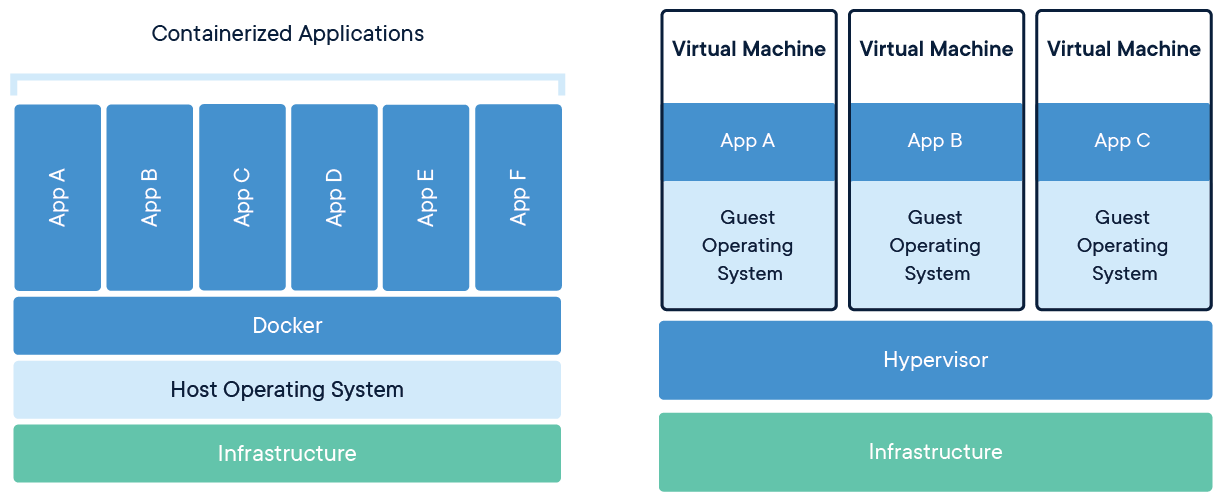
\includegraphics[width=\linewidth]{figures/docker-containerized-and-vm-transparent-bg.png}
\end{frame}
%---------------------------------------------------------

%---------------------------------------------------------
\subsection{Virtual Machines}
\begin{frame}
	\frametitle{Virtual Machines}
	\begin{itemize}
		\item Virtual machines (VMs) are an abstraction of physical hardware, turning one server into many servers.
		\item The hypervisor allows multiple VMs to run on a single machine.
		\item Each VM includes a full copy of an operating system, the application, necessary binaries, and libraries - taking up tens of GBs.
		\item VMs can also be slow to boot.
	\end{itemize}
\end{frame}
%---------------------------------------------------------

%---------------------------------------------------------
\subsection{Containers}
\begin{frame}
	\frametitle{Containers}
	\begin{itemize}
		\item Containers are an abstraction at the app layer that packages code and dependencies together.
		\item Multiple containers can run on the same machine and share the OS kernel with other Containers, each running as isolated processes in userspace.
		\item Containers take up less space than VMs (container images are typically tens of MBs in size), can handle more applications, and require fewer VMs and Operating systems. 
	\end{itemize}
\end{frame}
%---------------------------------------------------------

%---------------------------------------------------------
\subsection{Container-based virtualization Solutions}
\begin{frame}
	\frametitle{Container-based virtualization Solutions}
	\begin{itemize}
		\item \textbf{Docker} is the most popular, and we will explain briefly.
		\item \textbf{OpenVZ}
		\item \textbf{LXC} Linux containers 
	\end{itemize}
\end{frame}
%---------------------------------------------------------

%---------------------------------------------------------
\subsection{References}
\begin{frame}
	\frametitle{References}
	\begin{itemize}
		\item \href{https://www.docker.com/resources/what-container}{Docker - What is a container?}
		\item \href{https://openvz.org/}{OpenVZ}
		\item \href{https://linuxcontainers.org/}{Linux Containers}
	\end{itemize}
\end{frame}
%---------------------------------------------------------

%---------------------------------------------------------
\end{document}
